\documentclass[conference]{IEEEtran}
\usepackage[cmex10]{amsmath}
\usepackage{xcolor}
\usepackage{graphicx}
\hyphenation{op-tical net-works semi-conduc-tor}

\begin{document}
\title{LNA Design\\ECE 432 Microwave Circuit Design II}
\author{\IEEEauthorblockN{Jackson Pugh}
\IEEEauthorblockN{Michael Woodruff}
\IEEEauthorblockA{Portland State University\\
Portland, OR 97207}}
\maketitle
\IEEEpeerreviewmaketitle
\section{LNA Design}
The LNA design is comprised of Minicircuit's low noise SAV-541+ transistor.  Consideration of a suitable bias network is required for gain and stability.  Looking at the SAV-541+ datasheet\cite{sav541datasheet}, a good place to bias the transistor is $I_{DS}$ = 60 mA at $V_{DS}$ = 3 V.  The recommended application circuit provided in the datasheet is used in the design.   The BJT current mirror helps draw $I_{DS}$ to 60 mA.  The supply power was chosen to be 3.7 V (instead of 3.3 V) due to the 0.7 V drop from the BJT current mirror.

Figure~\ref{fig:dccircuit} shows the bias network for the transistor circuit.  Figure~\ref{fig:dcvalues} shows the DC measurements of the parameters of interest.  Figure~\ref{fig:sparamresult} shows the S-Parameter comparison between the bias network circuit and the manufacturer S2P data.  The bias network shows little discrepency but works as expected.

\begin{figure}[!h]
\centering
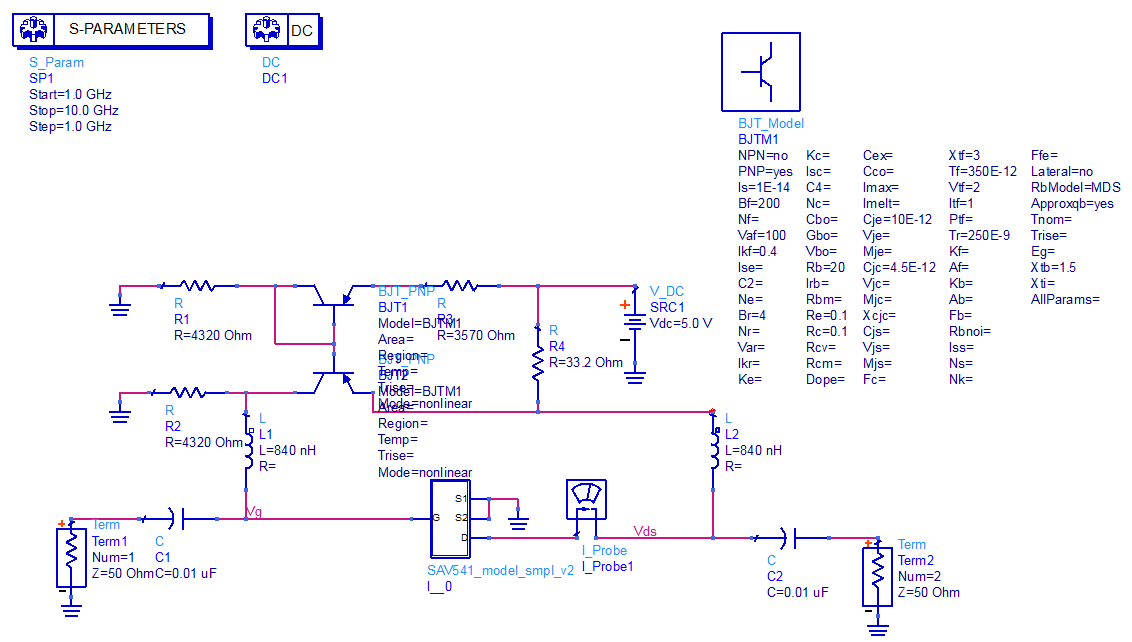
\includegraphics[scale=0.29]{pics/DCBiasNetwork.png}
\caption{DC bias network for the SAV-541+ transistor.}
\label{fig:dccircuit}
\end{figure}

\begin{figure}[!h]
\centering
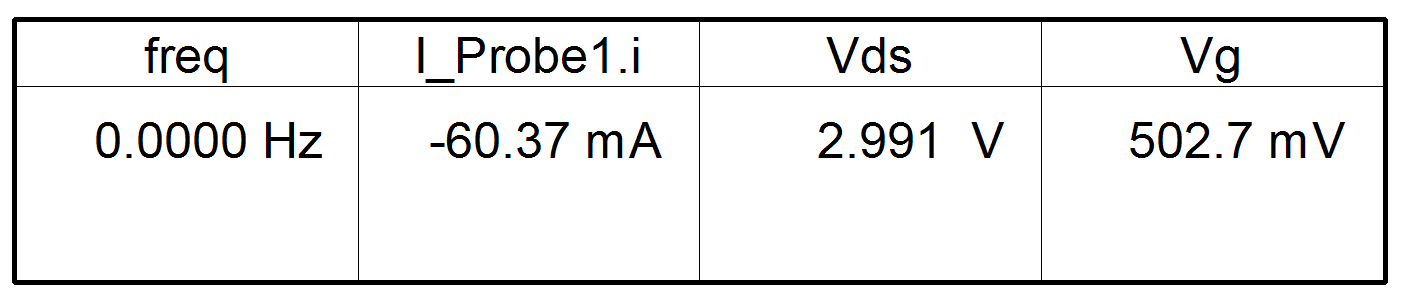
\includegraphics[scale=0.21]{pics/DCBiasResults.png}
\caption{Current and voltage  parameters from the DC bias network for the SAV-541+ transistor.}
\label{fig:dcvalues}
\end{figure}

\begin{figure}[!h]
\centering
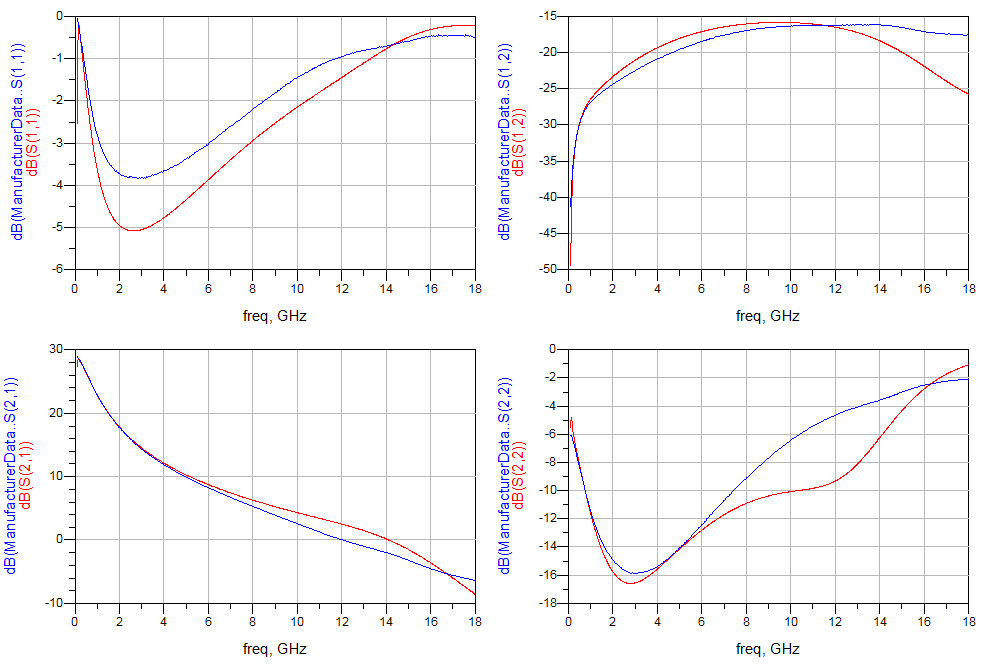
\includegraphics[scale=0.35]{pics/SParameterComparison.png}
\caption{S-Parameter simulation result comparison between the bias network and the manufacturer S2P data file.}
\label{fig:sparamresult}
\end{figure}

Figure~\ref{fig:designguide} shows various information provided by the ADS amplifier design guide tool.  Observing the Stability Factor, K ($mu_{source}$/$mu_{load}$) graph, the circuit is potentially unstable below around 4 GHz.  Thus, stabilizing resistors will be necessary in order to make the transistor unconditionally stable between 2.4 - 2.6 GHz (the intended frequency range).

\begin{figure}[!h]
\centering
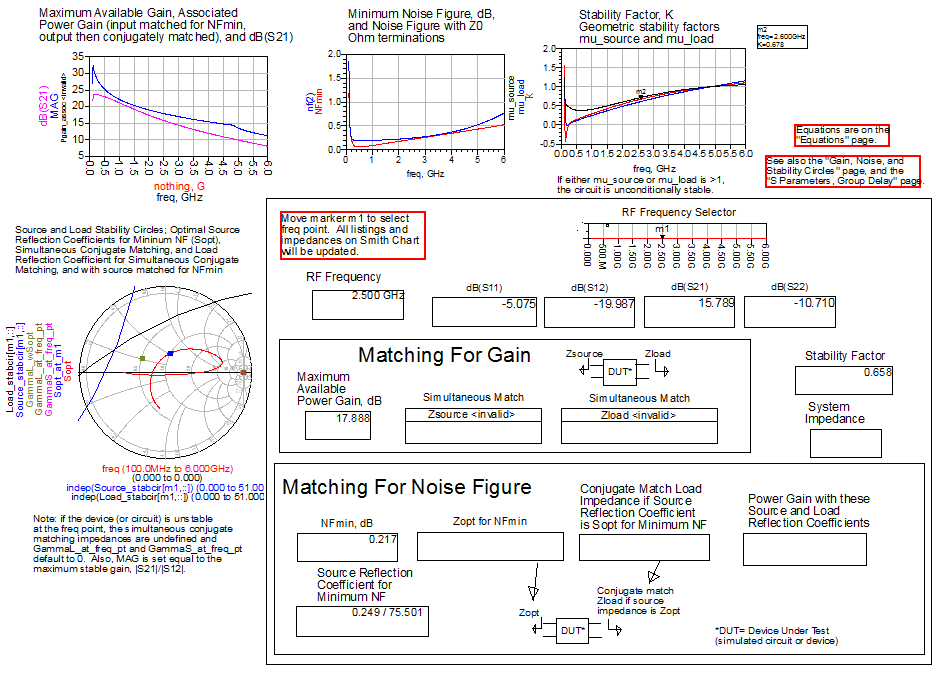
\includegraphics[scale=0.35]{pics/DesignGuideUnoptimized.png}
\caption{Amplifier design guide generated in ADS for the bias network for the SAV-541+ transistor.}
\label{fig:designguide}
\end{figure}

Figure~\ref{fig:designcuidecircuitstabilized} shows added feedback to the transistor used to stablize it unconditionally (under 3 GHz).  After tweaking the circuit for stability, Figure~\ref{fig:designcuidesimulationstabilized} shows the Design Guide for the stabilzed circuit. It shows the circuit is unconditionally stable with a gain of 12.225 dB.

\begin{figure}[!h]
\centering
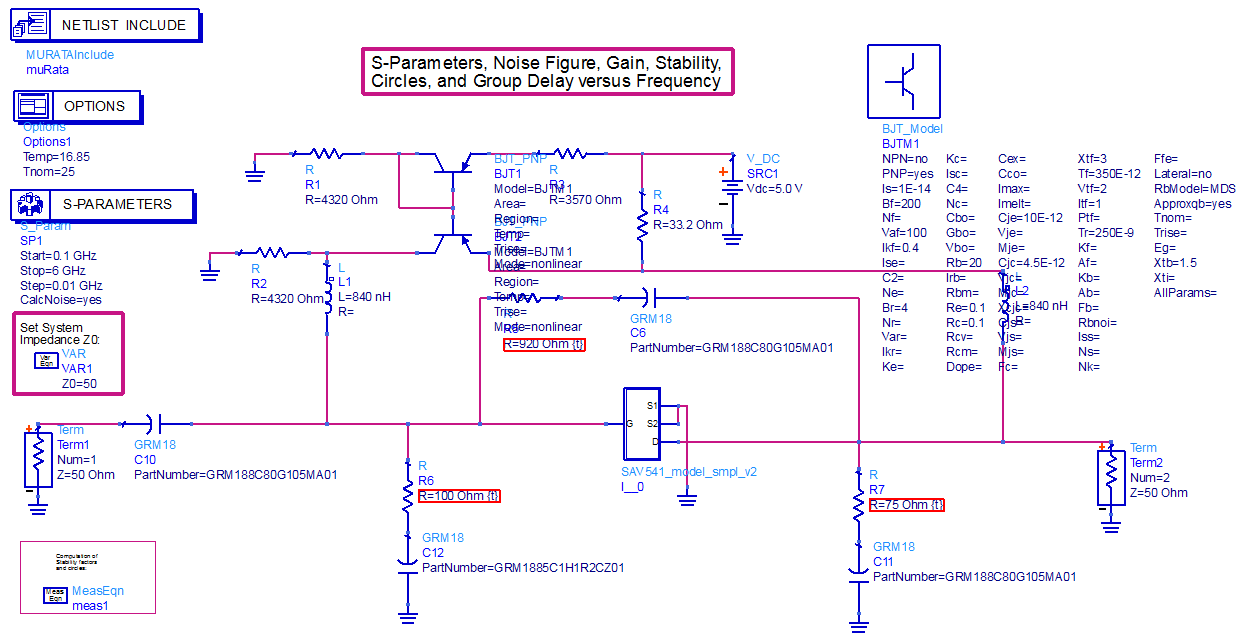
\includegraphics[scale=0.26]{pics/DesignGuideStablizedCircuit.png}
\caption{Stabilized transistor bias circuit for the SAV-541+ using feedback and stabilizing resistors.}
\label{fig:designcuidecircuitstabilized}
\end{figure}

\begin{figure}[!h]
\centering
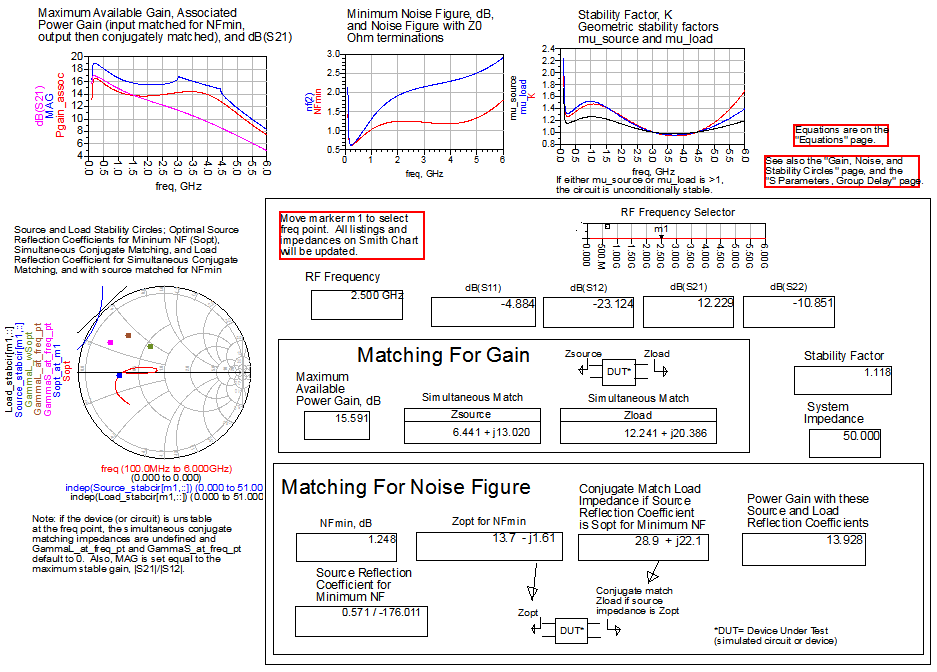
\includegraphics[scale=0.35]{pics/DesignGuideStablizedSimulation.png}
\caption{Amplifier design guide generated in ADS for the bias network for the SAV-541+ transistor.}
\label{fig:designcuidesimulationstabilized}
\end{figure}

The circuit now needs transmission line in order to be able to manufacture the board.  As expected, adding transmission line to the circuit caused the transistor to become potentially unstable.  Thus, it was required to tune the feedback components again.  Figure~\ref{fig:finalstabcircuit} shows the finalized stabilizing circuit for the SAV-541+ transistor.  Figure~\ref{fig:finalstabsimulation} shows the design guide plots.  By observing the $mu_{load}$/$mu_{source}$, the circuit will be unconditionally stable between 0.1 GHz - 6 GHz.  In addition, the gain is above 10 dB.

\begin{figure}[!h]
\centering
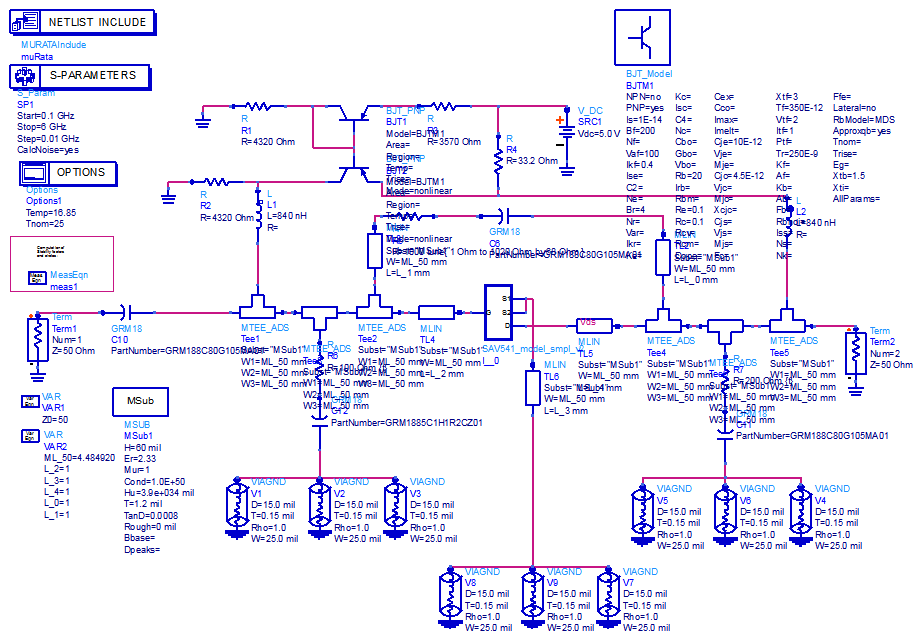
\includegraphics[scale=0.35]{pics/FinalStabilizingCircuit.png}
\caption{Final stabilizing circuit for the SAV-541+ transistor.}
\label{fig:finalstabcircuit}
\end{figure}

\begin{figure}[!h]
\centering
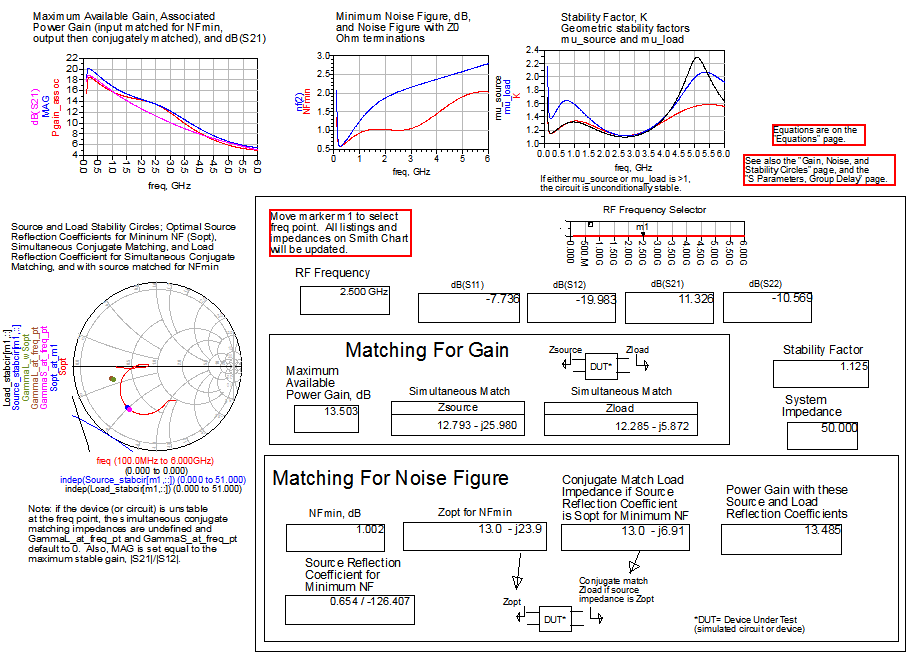
\includegraphics[scale=0.35]{pics/FinalStabilizingSimulation.png}
\caption{ADS design guide simulation results for the stabilizing circuit for the SAV-541+ transistor.}
\label{fig:finalstabsimulation}
\end{figure}

Figure~\ref{fig:lnaLayout} shows the layout which will be used to manufacture the physical board.
\begin{figure}[!h]
\centering
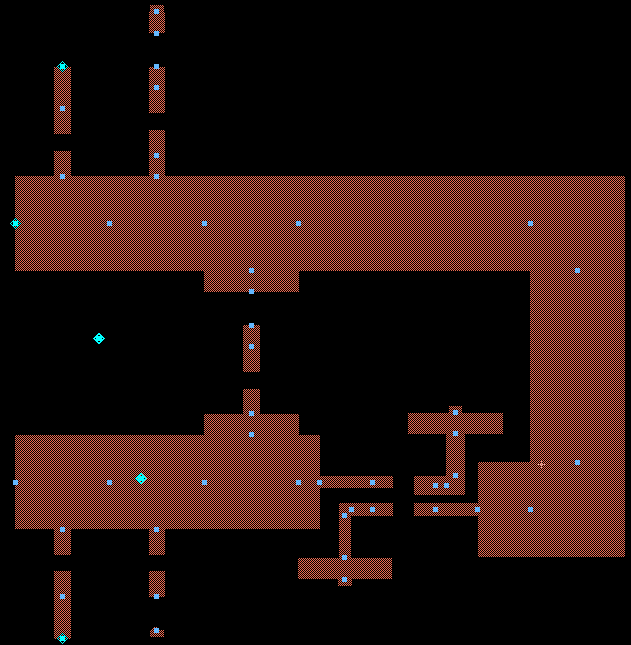
\includegraphics[scale=0.35]{LNApics/LNAlayout.png}
\caption{SAV-541+ transistor layout.}
\label{fig:lnaLayout}
\end{figure}

\begin{thebibliography}{1}
\bibitem{payne}
K. Payne, "Practical RF Amplifier Design Using the Available Gain Procedure and the Advanced Design System EM/Circuit Co-Simulation Capability," Agilent Technologies (5990-3356EN), 2008.
\bibitem{sav541datasheet}
Minicircuit SAV-541+ Datasheet
\end{thebibliography}
\end{document}